\begin{tikzpicture}
\node (overview) at (-10,5) {        \begin{tikzpicture}[]
        \centering
        \begin{axis}[
        view={40}{35},
            ylabel={$p$},
            xlabel={$Sk$},
			zlabel={$\Delta U^+$},
			ztick={5.5,6,6.5,7,7.5},
            %ymin=0, ymax=1,
            width=.6\textwidth,
            height=.4\textwidth,
            label style={font=\footnotesize},
            tick label style={font=\footnotesize}
            ]
 %           \addplot3 [
%            blue,dashed,thick,no marks
%            ]
%            coordinates{
%            (0,-2,6.326)			%
%			(0.48,-2,6.994)%
%			(0.48,-1,7.336)
%			(0,-1,6.656)
%			(-0.48,-1,6.096)
%			(-0.48,-2,5.789)
 %           (0,-2,6.326)
%			};
%			\addplot3 [
 %5           red,dashed,thick, no marks
  %          ]
   %         coordinates{
    %        
    % 5       (0,-2,5.912)
	%		(0.48,-2,6.607)
	%		(0.48,-1,7.262)
	%5		(0,-1,6.530)
	%5		(-0.48,-1,6.075)
	%		(-0.48,-2,5.458)
	%5		(0,-2,5.912)
     %       };
                        \addplot3 [
            black,mark=x,thick, mark size=3pt
            ]
            coordinates{
            (0,-2,6.20)			
			(0.48,-2,6.9176)
			(0.48,-1,7.3502)
			(0,-1,6.56)
			(-0.48,-1,5.87)
			(-0.48,-2,5.8034)
            (0,-2,6.20)
			};
			\addplot3 [
            gray!60,mark=x,thick, mark size=3pt
            ]
            coordinates{
            
            (0,-2,5.8764)
			(0.48,-2,6.8720)
			(0.48,-1,7.3415)
			(0,-1,6.5891)
			(-0.48,-1,6.0625)
			(-0.48,-2,5.5765)
			(0,-2,5.8764)
            };
                                    \addplot3 [
            black,mark=x,thick, mark size=3pt
            ]
            coordinates{
            (0,-2,6.20)			
			(0,-1,6.56)
			};
			\addplot3 [
            gray!60,mark=x,thick, mark size=3pt
            ]
            coordinates{
            (0,-2,5.8764)
			(0,-1,6.5891)
            };
        \end{axis}
        \end{tikzpicture}};
\node (caption_overview) [right=of overview,align=left] {(a) Overview of results.\\Black: $\lambda_0=0.8H$, gray: $\lambda_0=1.6H$};
\node (Sk) at (-15,0) {        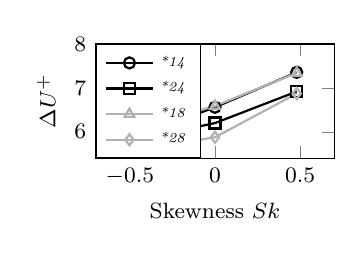
\begin{tikzpicture}[]
        \centering
        \begin{axis}[
            ylabel={$\Delta U^+$},
            xlabel={Skewness $Sk$},
            ymin=5.4, ymax=8,
			xmax=0.7,
			xmin=-0.7,
            width=.38\textwidth,
            height=.25\textwidth,
            label style={font=\footnotesize},
			legend style={font=\tiny,at={(0,1)},anchor=north west},
            tick label style={font=\footnotesize}
            ]
			\addplot [
            black,solid,thick,mark=o,
            ]
            coordinates{
            (-0.48, 5.87)
            (0, 6.56)
            (0.48, 7.3562)
            };
			\addlegendentry{\textit{*14}}
			\addplot [
            black,solid,thick,mark=square,
            ]
            coordinates{
            (-0.48, 5.8034)
            (0, 6.20)
            (0.48, 6.9176)
            };
			\addlegendentry{\textit{*24}}
			\addplot [
            gray!60,solid,thick,mark=triangle,
            ]
            coordinates{
            (-0.48, 6.0625)
            (0, 6.5891)
            (0.48, 7.3415)
            };
			\addlegendentry{\textit{*18}}
						\addplot [
            gray!60,solid,thick,mark=diamond,
            ]
            coordinates{
            (-0.48, 5.5765)
            (0, 5.8764)
            (0.48, 6.8720)
            };
			\addlegendentry{\textit{*28}}
        \end{axis}
        \end{tikzpicture}};
\node (caption_sk) [below=of Sk,align=left] {(b) $\Delta U^+$ as a function of $Sk$.\\Black: $\lambda_0=0.8H$, gray: $\lambda_0=1.6H$};
\node (p) at (-5,0) {        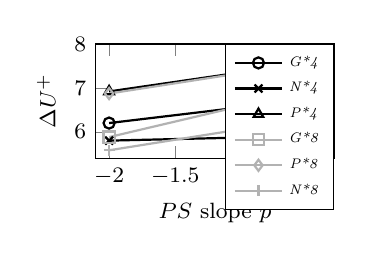
\begin{tikzpicture}[]
        \centering
        \begin{axis}[
            ylabel={$\Delta U^+$},
            xlabel={$PS$ slope $p$},
            ymin=5.4, ymax=8,
			xmax=-0.3,
			xmin=-2.1,
			xtick={-2,-1.5,...,-0.4},
            width=.38\textwidth,
            height=.25\textwidth,
            label style={font=\footnotesize},
			legend style={font=\tiny,at={(1,1)},anchor=north east},
            tick label style={font=\footnotesize}
            ]
			\addplot [
            black,solid,thick,mark=o,
            ]
            coordinates{
            (-1, 6.56)
            (-2, 6.20)
            };
			\addlegendentry{\textit{G*4}}
			
									\addplot [
           black,solid,thick,mark=x,
            ]
            coordinates{
            (-1, 5.87)
            (-2, 5.80)
            };
			\addlegendentry{\textit{N*4}}
									\addplot [
           black,solid,thick,mark=triangle,
            ]
            coordinates{
            (-1, 7.3562)
            (-2, 6.92)
            };
			\addlegendentry{\textit{P*4}}
			
			\addplot [
            gray!60,solid,thick,mark=square,
            ]
            coordinates{
            (-1, 6.59)
            (-2, 5.88)
            };
			\addlegendentry{\textit{G*8}}

						\addplot [
            gray!60,solid,thick,mark=diamond,
            ]
            coordinates{
            (-1, 7.34)
            (-2, 6.8720)
            };
			\addlegendentry{\textit{P*8}}

						\addplot [
            gray!60,solid,thick,mark=+,
            ]
            coordinates{
            (-1, 6.06)
            (-2, 5.58)
            };
			\addlegendentry{\textit{N*8}}
        \end{axis}
        \end{tikzpicture}};
\node (caption_p) [below=of p,align=left] {(c) $\Delta U^+$ as a function of $p$.\\Black: $\lambda_0=0.8H$, gray: $\lambda_0=1.6H$};
\node (lambda) at (-10.5,-6.5) {        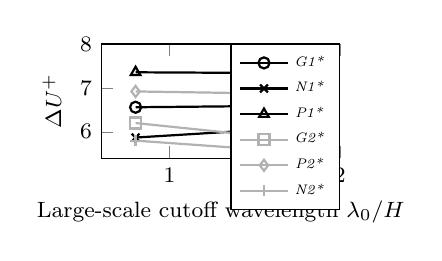
\begin{tikzpicture}[]
        \centering
        \begin{axis}[
            ylabel={$\Delta U^+$},
            xlabel={Large-scale cutoff wavelength $\lambda_0/H$},
            ymin=5.4, ymax=8,
			xmax=2,
			xmin=0.6,
            width=.38\textwidth,
            height=.25\textwidth,
            label style={font=\footnotesize},
			legend style={font=\tiny,at={(1,1)},anchor=north east},
            tick label style={font=\footnotesize}
            ]
			\addplot [
            black,solid,thick,mark=o,
            ]
            coordinates{
            (0.8, 6.56)
            (1.6, 6.59)
            };
			\addlegendentry{\textit{G1*}}
			
									\addplot [
            black,solid,thick,mark=x,
            ]
            coordinates{
            (0.8, 5.87)
            (1.6, 6.06)
            };
			\addlegendentry{\textit{N1*}}
			
						\addplot [
            black,solid,thick,mark=triangle,
            ]
            coordinates{
            (0.8, 7.3562)
            (1.6, 7.34)
            };
			\addlegendentry{\textit{P1*}}
			
			
			
			\addplot [
            gray!60,solid,thick,mark=square,
            ]
            coordinates{
            (0.8, 6.20)
            (1.6, 5.88)

            };
			\addlegendentry{\textit{G2*}}

						\addplot [
            gray!60,solid,thick,mark=diamond,
            ]
            coordinates{
            (0.8, 6.92)
            (1.6,6.8720)
            };
			\addlegendentry{\textit{P2*}}

						\addplot [
            gray!60,solid,thick,mark=+,
            ]
            coordinates{
            (0.8, 5.80)
            (1.6, 5.58)
            };
			\addlegendentry{\textit{N2*}}
        \end{axis}
        \end{tikzpicture}};
\node (caption_lambda) [below=of lambda,align=left] {(d) $\Delta U^+$ as a function of $\lambda_0$.\\Black: $p=-1$, gray: $p=-2$};





%\node (good) [right=of bad] {\includegraphics[width=4cm]{example-image-b}};

\node (OL)  at (-12,4) {};
\node (OR)  at (-8,4) {};
\node (OB)  at (-10,3) {};
\node (Sk)  at (-15,2) {};
\node (p)  at (-5,2) {};
\node (lambda)  at (-10,-4.5) {};
\draw [ultra thick,black,->] (OL) to[bend right] (Sk);
\draw [ultra thick,black,->] (OR) to[bend left] (p);
\draw [ultra thick,black,->] (OB) to (lambda);
%\draw [ultra thick,magenta,->] (a) to[bend left] (b);
\end{tikzpicture}